\newpage
\subsection{UC3 - Modifica Metadati}
\label{sub:uc2}

%TODO: Add correct image
\begin{figure}[h]
    \centering
    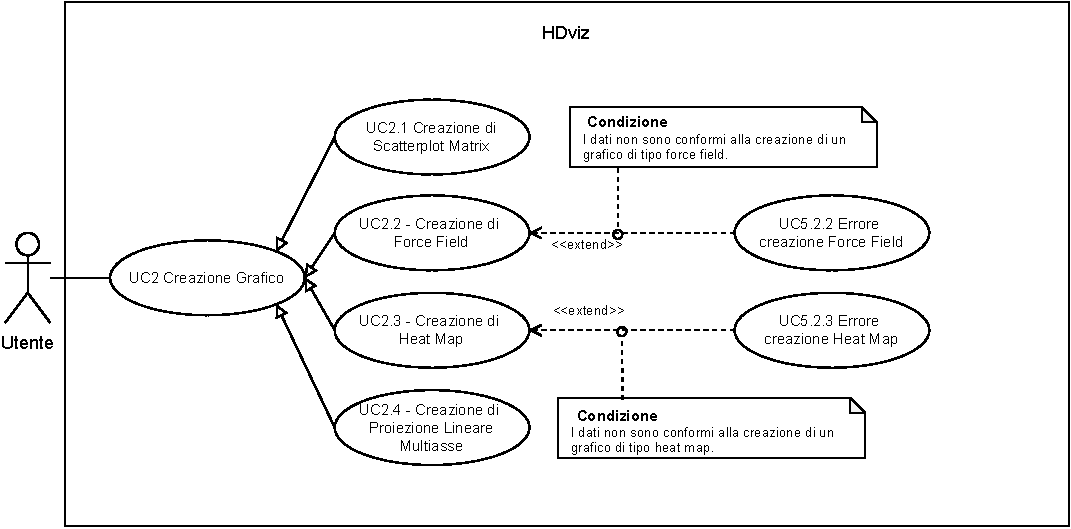
\includegraphics[width=0.8\textwidth]{componenti/casi-duso/diagrammi/UC2.pdf}
    \caption{Diagramma rappresentante UC2}
    \label{fig:UC2}
\end{figure}


\begin{itemize}
    \item \textbf{Descrizione}: L’utente vuole modificare uno o più metatag attualmente assegnati al dataset.
	
    \item \textbf{Attore primario}: Utente.
    
    \item \textbf{Precondizione}:   Nel programma è stato importato un dataset dotato di metatag per ogni
                                    colonna dei dati.

    \item \textbf{Postcondizione}:  Vengono aggiornati i metadati del dataset.

	\item \textbf{Scenario principale}:
		\begin{enumerate}
			\item L'utente decide se effettuare modifiche ai metatag e le effettua.
        \end{enumerate}

\end{itemize}
